\section{Einführung}

Eine Idee von Grund auf nach ``agile'' und ``lean'' Prinzipien aufbauen - Dies ist die Grundiee dieser Arbeit. Sie beschäftigt sich mit allen Stufen eines innovativen Projekts von Ideensuche, über Kundeinterviews bis zu modernen Entwicklungstools und iterativem Release. In diesem ersten Teil der Arbeit wird unser Vorgehensmodell aufgezeigt und die Spielregeln im Team erläutert.

\subsection{Vorgehen}
Abbildung \ref{fig:vorgehen} zeigt das Vorgehensmodell, an das wir uns im Rahmen dieses Projekts halten. Dieses verbindet die beiden Modelle ``Design Thinking'' und ``Lean Startup''. Im ersten Schritt werden die Schritte von Design Thinking durchlaufen. Diese können auch iterativ sein und haben am Ende das Ziel eine Idee bzw. ein Problem validiert zu haben. Anhand dieser Idee kann anschliessend im ``Build - Measure - Learn'' Zyklus nach \citet{ries2014lean} ein Produkt iterativ entwickelt werden. Im Prozess wollen wir uns vor allem auf die ersten beiden Stadien \textit{Design Thinking} und \textit{Lean Startup} konzentrieren. Der Teilbereich \textit{Agile} werden wir wahrscheinlich noch nicht erreichen, da es sich dort bereits um eine relativ gut etablierte Idee bzw. Lösung handeln muss, um wirklich effektiv in diesem Bereich arbeiten zu können.

\begin{figure}[H]
    \centering
    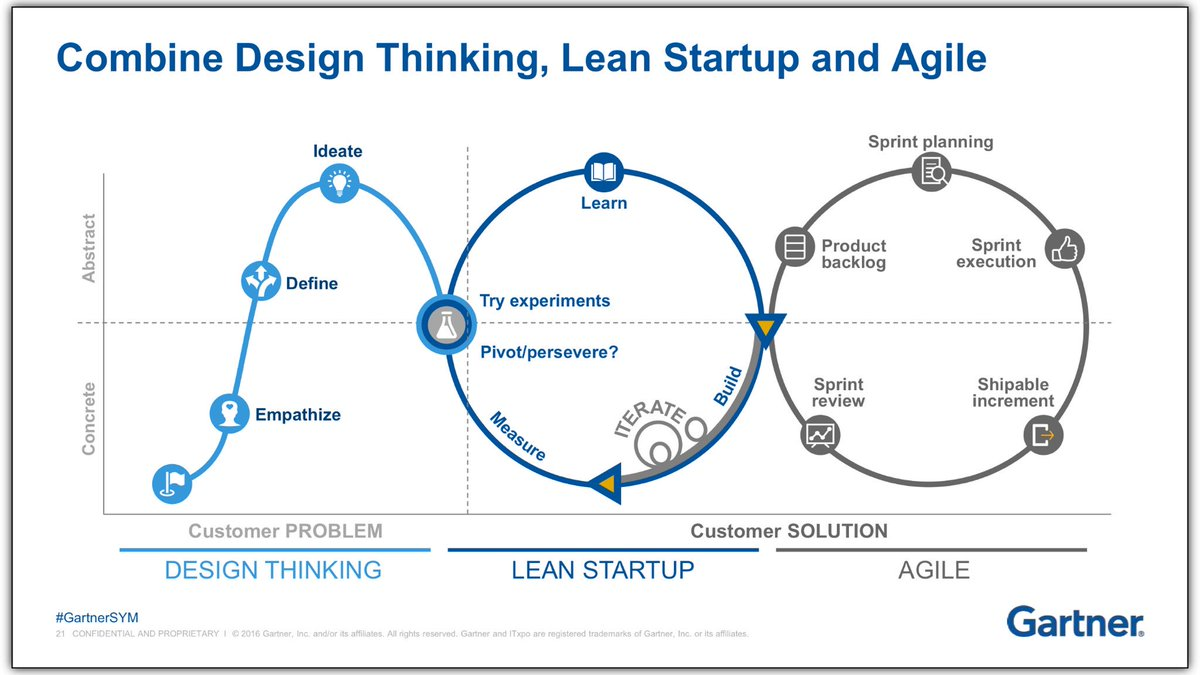
\includegraphics[width=\textwidth]{images/LeanStartup.png}
    \caption{Vorgehensmodell}
    \label{fig:vorgehen}
\end{figure}

\subsection{Spielregeln betreffend Zusammenarbeit}
Um die Zusammenarbeit im Team so reibungslos wie möglich gestalten zu können haben wir die folgenden ``Spielregeln'' aufgestellt, an welche wir uns während des ganzen Projekts halten möchten.
\begin{enumerate}
\item Tools:
    \begin{itemize}
        \item [i.]Projektplanung: Trello
        \item [ii.]Schreiben von Dokumenten: Overleaf
        \item [iii.]Versionierung: Git/Gitlab
    \end{itemize}
\item Vorgehen:
    \begin{itemize}
        \item [i.]Abgabe der Dokumente ist jeweils Samstagabend 
        \newline(36h vor der nächsten PVA)
        \item[-]Der jeweilige Auftrag sollte bis Freitagmittag gemacht sein, sodass wir
        noch Zeit für Reviews haben.
        \item [ii.]Dedizierte Reviewers (noch zu bestimmen)
    \end{itemize}
\item Aufträge bereits unter dem Semester jeweils verbessern / Feedback einbauen und nicht erst am Ende des Semesters vor der Abgabe.
\item Klare Rollen im Team bestimmen: Wer plant? Wer entwirft Architektur? 
Umsetzung und Schreiben der Arbeiten auf alle aufteilen, jedoch ist es immer gut, wenn für diese beiden Teile jemand verantwortlich ist.


Diese Spielregeln sollen von allen Gruppenmitgliedern eingehalten werden. Es können im Laufe des Projektes auch noch weitere Spielregeln hinzugenommen werden.
\end{enumerate}